\documentclass{standalone}
\usepackage{tikz}             % TikZ and PGF
\title{main setup}

% Vector Styles
\tikzstyle{load}   = [ultra thick,-latex]
\tikzstyle{stress} = [-latex]
\tikzstyle{dim}    = [latex-latex]
\tikzstyle{axis}   = [-latex,black!55]

% Drawing Views
\tikzstyle{isometric}=[x={(0.610cm,-0.410cm)},y={(0cm,0.820cm)},z={(-0.990cm,-0.410cm)}]
\tikzstyle{dimetric} =[x={(0.935cm,-0.118cm)},y={(0cm,0.943cm)},z={(-0.354cm,-0.312cm)}]
\tikzstyle{dimetric2}=[x={(0.935cm,-0.118cm)},z={(0cm,0.943cm)},y={(+0.354cm,+0.312cm)}]
\tikzstyle{trimetric}=[x={(0.926cm,-0.207cm)},y={(0cm,0.837cm)},z={(-0.378cm,-0.507cm)}]

\begin{document}
  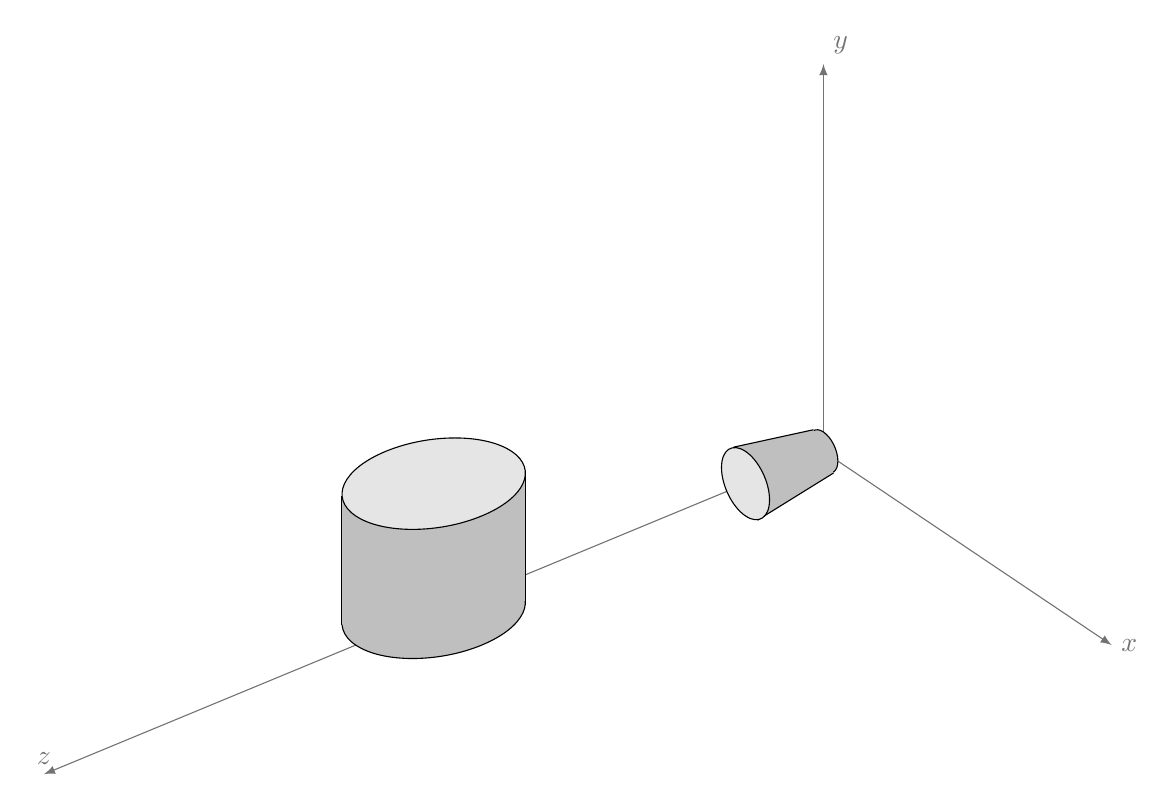
\begin{tikzpicture}[isometric]
	% Coordinates
	\coordinate (O) at (0,0,0);
  \draw[axis] (O) -- ++(6,0,0) node[right] {$x$};
  \draw[axis] (O) -- ++(0,6,0) node[above right] {$y$};
  \draw[axis] (O) -- ++(0,0,10) node[above] {$z$};
				
	% Detector			
	\draw[fill=gray!50] (0,0,0) circle (0.3);
  
	\fill[fill=gray!50] (-0.21,0.23,0) -- (-0.25,0.44,1) -- (0.25,-0.44,1) -- (0.21,-0.23,0) -- cycle;
	
	\draw (-0.21,0.23,0) -- (-0.25,0.44,1); 
	%.. controls (-0.23,0.25,0.5) ..
	\draw (0.21,-0.23,0) -- (0.25,-0.44,1); 

	\draw[fill=gray!20] (0,0,1) circle (0.5);
	
	% Source
	\draw[fill=gray!50] (-1,0,5) .. 
    	controls (-1,0,5.555) and (-0.555,0,6) .. (0,0,6) .. 
    	controls (0.555,0,6) and (1,0,5.555) .. (1,0,5) .. 
    	controls (1,0,4.445) and (0.555,0,4) .. (0,0,4) .. 
    	controls (-0.555,0,4) and (-1,0,4.445) .. (-1,0,5) -- cycle;
    \fill[fill=gray!50] (-.5,0,5.87) -- (.5,0,4.13) -- (.5,2,4.13) -- (-.5,2,5.87) -- cycle;
	\draw (-.5,0,5.87) -- (-.5,2,5.87);
	\draw (.5,0,4.13) -- (.5,2,4.13);
	\draw[fill=gray!20] (-1,2,5) .. 
    	controls (-1,2,5.555) and (-0.555,2,6) .. (0,2,6) .. 
    	controls (0.555,2,6) and (1,2,5.555) .. (1,2,5) .. 
    	controls (1,2,4.445) and (0.555,2,4) .. (0,2,4) .. 
    	controls (-0.555,2,4) and (-1,2,4.445) .. (-1,2,5) -- cycle;
	
    
    
	
	%\draw (-0.46,-0.2,-0.5) -- ++(0,0,0.5);
  		
		%\draw[fill=gray!10] (O) circle (0.2);
   % \fill[fill=gray!10] (-0.175,-0.1,0) -- (0.175,0.1,0) -- ++(0,0,4) -- (-0.175,-0.1,4) -- cycle;
   % \draw (-0.175,-0.1,0) -- ++(0,0,4);
   % \draw (0.175,0.1,0) -- ++(0,0,4) node[right,midway] {Steel Post};
  %  \draw (4,0,3.95) -- ++(0,0,-1);

 %   \draw[fill=gray!20] (-0.25,-0.25,5) -- (4,-0.25,5) -- (4,+0.25,5) -- (-0.25,+0.25,5) -- cycle; 
 %   \draw[fill=gray!50] (+4.00,-0.25,4) -- (4,+0.25,4) -- (4,+0.25,5) -- (+4.00,-0.25,5) -- cycle; 
%    \draw (4.05,0,4) -- ++(1,0,0);
  %  \draw (4.05,0,5) -- ++(1,0,0);
  %  \draw[dim] (4.5,0,0) -- ++(0,0,4) node[midway,right] {$h_1$};
  %  \draw[dim] (4.5,0,4) -- ++(0,0,1) node[midway,right] {$h_2$};
  %  \draw[dim] (0,0,3.4) -- ++(4,0,0) node[midway,below] {$b_2$};
  %  \coordinate (P) at (2,-0.25,4.5);
  %  \draw (P) -- ++(0,0,0.25);
   % \draw (P) -- ++(0.25,0,0);

   
  \end{tikzpicture} %
\end{document}